\section{Inference}

We use Markov chain Monte Carlo to sample from the posterior distribution of our parameters.\footnote{TODO: Describe why EM is hard.} % Note that approaches such as EM are difficult since the form of the likelihood does not admit an analytic expression for the expected complete data log likelihood.

\subsection{Sampling $\mathbf{z}$ given $\boldsymbol{\beta}$ and $\mathcal{A}$ }

We use Gibbs sampling to sample the latent class assignments $\mathbf{z}$ from the conditional distribution
\begin{align*}
p(z_r | \mathbf{z}_{-r},\mathcal{A},\alpha,\boldsymbol{\beta}) \propto&  p(\mathcal{A}|\mathbf{z},\boldsymbol{\beta}) p(z_r | \mathbf{z}_{-r},\alpha) \\
p(\mathcal{A}|\mathbf{z},\boldsymbol{\beta}) \propto &
\prod_{m=1}^M \lambda_{i_m,j_m}(t_m|\cdot)^{\mathbf{1}[r \in \{i_m,j_m\}]}  \prod_{(i,j) \in \mathcal{R}_r} \exp \{ -(t_m - t_{m-1}) \lambda_{ij}(t_m|\cdot)\}
\end{align*}
where $\mathcal{R}_r = \{(i,j) \in \mathcal{R}: r \in \{i,j\}\}$ is the set of dyads involving node $r$.
Under a CRP($\alpha$) prior, we have $p(z_i = k | z_{-i},\alpha) = n_k $ and $p(z_i = \mbox{new} |  z_{-i},\alpha) = \alpha$ where $n_k$ is the number of nodes assigned to cluster $k$.

\subsection{Sampling $\boldsymbol{\beta}$ given $\mathbf{z}$ and $\mathcal{A}$ }

For each block $(k,l)$ we need to sample the vector of parameters $\boldsymbol{\beta}_{k,l}$ from its posterior
\begin{align*}
p(\boldsymbol{\beta}_{k,l} | \mathcal{A}, \textbf{z}, \boldsymbol{\mu}, \boldsymbol{\sigma}) &\propto p(\boldsymbol{\beta}_{k,l} | \boldsymbol{\mu}, \boldsymbol{\sigma}) p( \mathcal{A}| \textbf{z}, \boldsymbol{\beta}) \\
p(\boldsymbol{\beta}_{k,l} | \mu, \sigma) &= \prod_{p=1}^Pp(\beta_{k,l,p}|\mu_p,\sigma_p^2)\\
p(\mathcal{A}|\mathbf{z},\boldsymbol{\beta}) &\propto \prod_{m=1}^M \lambda_{i_m,j_m}(t_m|\cdot)^{\mathbf{1}[(i_m,j_m) \in \mathcal{V}_{k,l}]}
\prod_{(i,j) \in \mathcal{V}_{k,l}} \exp \{ -(t_m - t_{m-1}) \lambda_{ij}(t_m|\cdot)\}
\end{align*}
where $\mathcal{V}_{k,l} = \{(i,j): z_{i} \in \{k,l\} \ \mbox{or} \ z_{j} \in \{k,l\} \}$ is the set of dyads with a sender in group $k$ and a recipient in $l$.  We sample each $\beta_{k,l,p}$ via slice sampling.

\subsection{Sampling $\mu$  and $\sigma$ given $\beta$ }

The inverse gamma distribution is a conjugate prior to a Gaussian distribution with known location parameter, thus $\sigma$ can be sampled from the conditional distribution
\begin{align}
\label{eqn:gibbs.sigma}
\sigma_p^2 &| \boldsymbol{\beta}, \mu_p,  \alpha_{\sigma}, \beta_{\sigma} \sim
 \mbox{Inv-Gamma}\left(\alpha_{\sigma} + \frac{K^2}{2}, \beta_{\sigma} + \frac{1}{2} \sum_{k=1}^K\sum_{l=1}^K (\beta_{k,l,p} - \mu_p)^2\right).
\end{align}
Each parameter $\mu_p$ can be sampled from its conditional distribution given $\sigma_p^2$ and the parameters $\boldsymbol{\beta}$,
\begin{align}
\label{eqn:gibbs.mu}
\mu_p | \boldsymbol{\beta},\sigma_p^2 &\sim \mbox{Normal}\left(\frac{1}{K^2}\sum_{k=1}^K \sum_{l=1}^K \beta_{k,l,p},\frac{ \sigma_p^2}{\sqrt{K^2}}\right).
\end{align}

\begin{figure}
\center
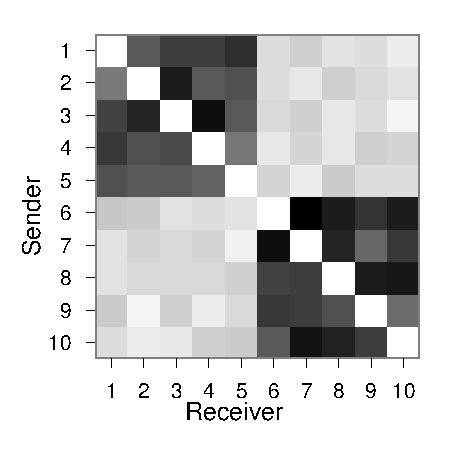
\includegraphics[width=1.6in]{../figs/synthetic/mat.pdf}
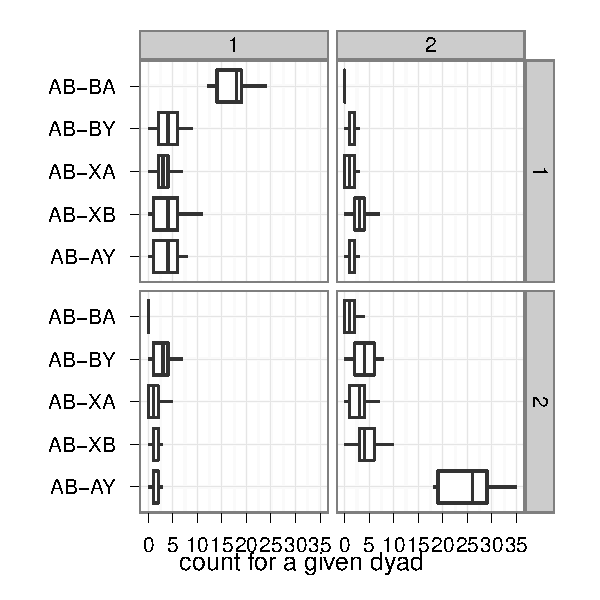
\includegraphics[width=2in]{../figs/synthetic/counts.pdf}
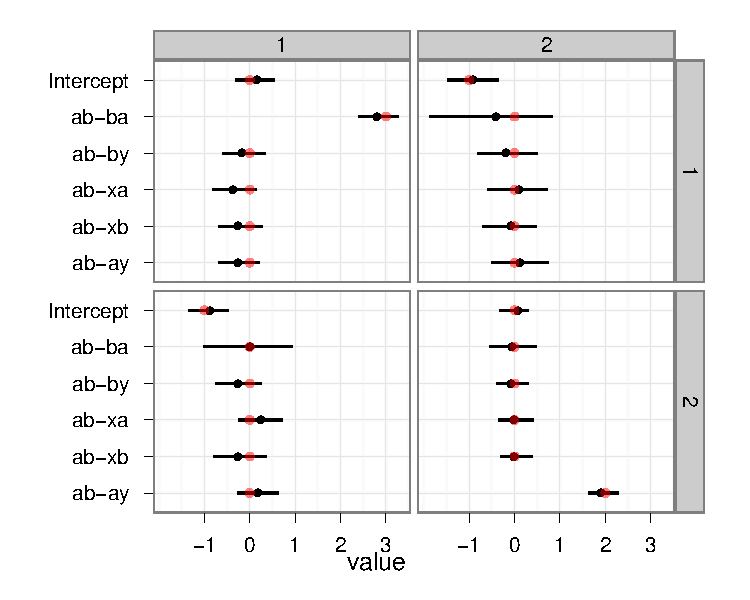
\includegraphics[width=1.8in]{../figs/synthetic/params-estimates.pdf}
\caption{Illustration of 2000 simulated events, as described in text. Left: Counts of each dyad. Center: Boxplot of distribution of participation counts across dyads.  The top left shows an increased propensity for reciprocity within cluster 1; bottom right shows more AB-AY events within cluster 2.  Right: Parameters (in red) and posterior credible intervals (in black).}
\label{fig:syncounts}
\end{figure}

\subsection{Hyperparameter settings}
In our experiments we use $\alpha=0.1$ and use Algorithm 8 from \cite{Neal2000} with 5 extra clusters drawn from the prior.\footnote{I also tried out a prior for cluster sizes such that $n_k \sim \mbox{NegBinom}(3,N/K)$, where $K$ is chosen a priori.  This aims for similarly sized groups.}
We set $\alpha_{\sigma}=3$ and $\beta_{\sigma}=1$ so that in the presence of little data we encourage shrinkage towards the upper level parameters $\mu$.  
As with other models, we note that the predictive accuracy of the model can depend on the hyperparameters.
